\section{User evaluation}
\label{sec:user_evaluation}

As said in the introduction of this chapter, this section deals with the user 
evaluation. In order to make a proper comparison between the presented systems 
several users have been guided through a demonstration of AdaptUI and a 
comparison with Imhotep. Besides, they have been questioned following the \ac{sus} 
guidelines.

\subsection{The \ac{sus} questionnaire}
\label{sec:sus}
The \ac{sus} (System Usability Scale)~\citep{sus} is a 10-item questionnaire 
developed by John Brooke in 1986 which gives an overview of satisfaction of 
users with software. Originally, it was conceived as a ``quick and dirty'' 
scale to collect the usability feedback from using systems similar to VT100 
Terminal applications (see the DEC VT100 video terminal in 
Figure~\ref{fig:vt100}).

\begin{figure}
\centering
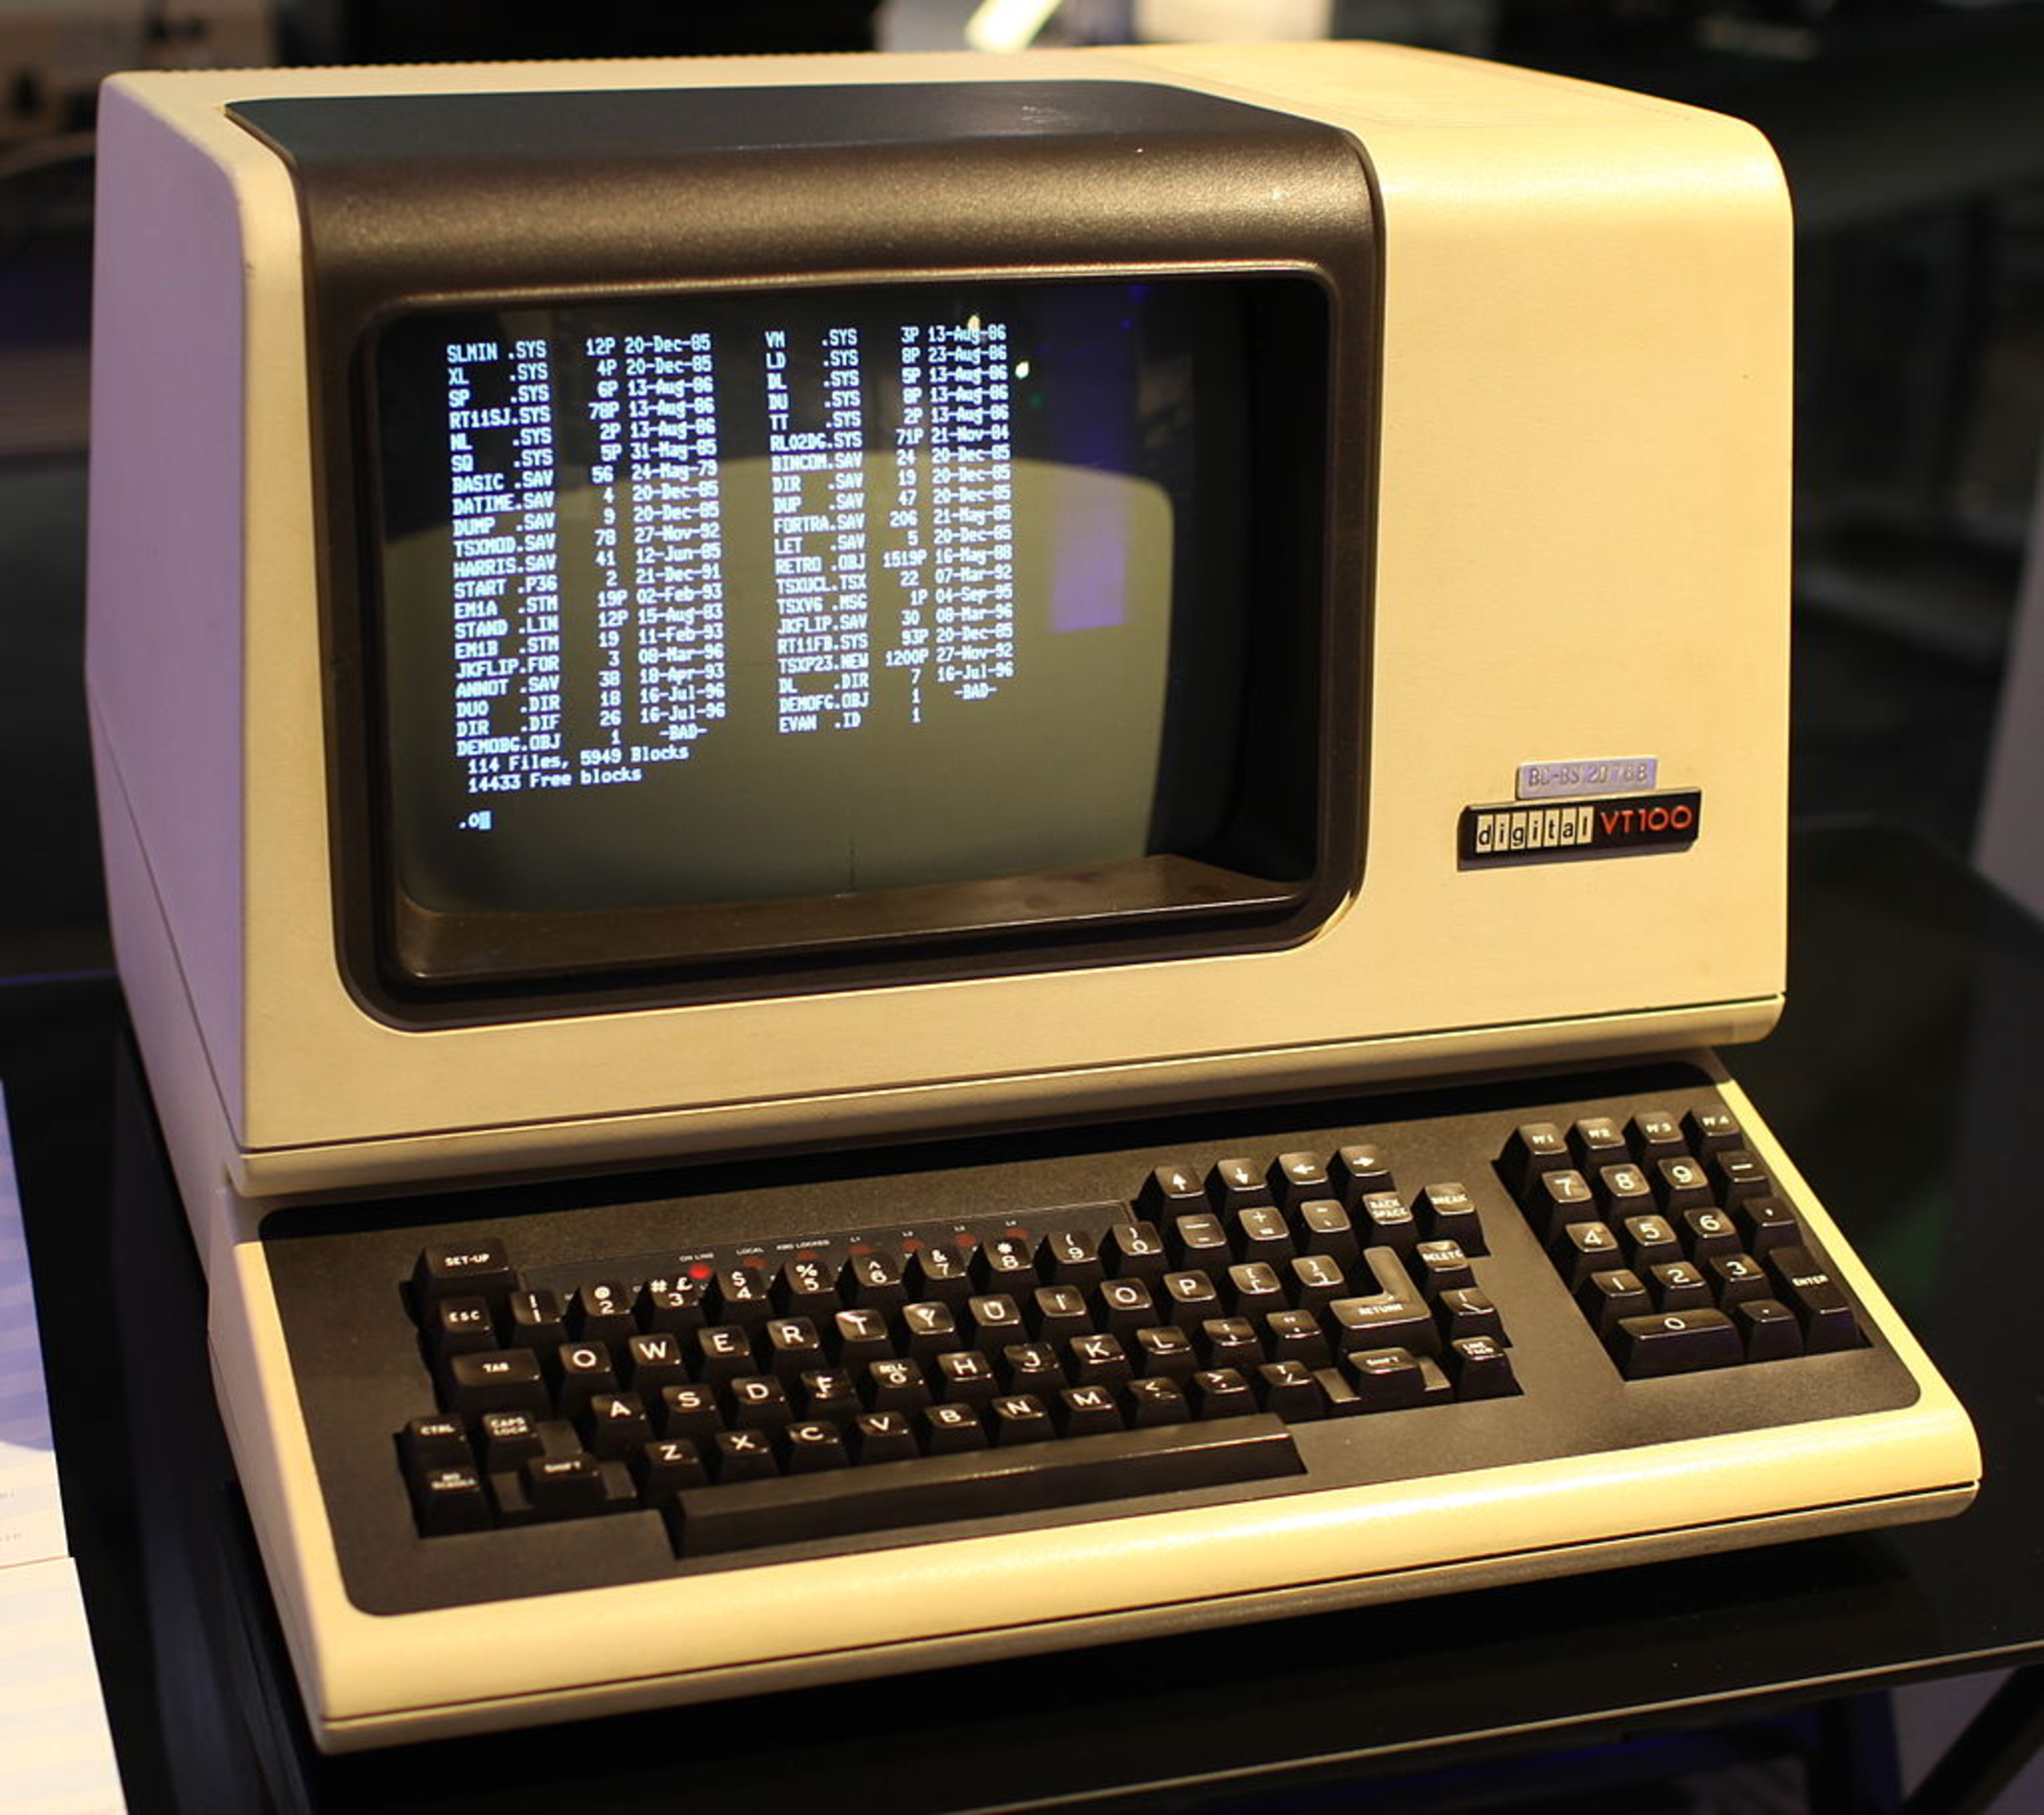
\includegraphics[width=0.65\textwidth]{vt100.pdf}
\caption{The Digital Equipment Corporation (DEC) VT100 video terminal, 
introduced in August 1978~\citep{vt100}.}
\label{fig:vt100}
\end{figure}

One of the \ac{sus} questionnaire main characteristics is its ability to collect
usability feedback through a 10 item questionnaire with 5 response options: 

\begin{enumerate}
 \item I think that I would like to use this system frequently.
 \item I found the system unnecessarily complex.
 \item I thought the system was easy to use.
 \item I think that I would need the support of a technical person to be able to
 use this system.
 \item I found the various functions in this system were well integrated.
 \item I thought there was too much inconsistency in this system.
 \item I would imagine that most people would learn to use this system very
 quickly.
 \item I found the system very cumbersome to use.
 \item I felt very confident using the system.
 \item I needed to learn a lot of things before I could get going with this
 system.
\end{enumerate}

To measure the resulting responses from the users, the formula described bellow
is applied: 

\begin{itemize}
 \item For odd items: subtract one from the user response.
 \item For even-numbered items: subtract the user responses from 5.
 \item This scales all values from 0 to 4 (with four being the most positive 
  response).
 \item Add up the converted responses for each user and multiply that total by 
  2.5. 
 This converts the range of possible values from 0 to 100 instead of from 0 to 
  40.
\end{itemize}

Thus, a figure between 0 and 100 is obtained, indicating the percentage of 
acceptance of the corresponding evaluated system. 
Figure~\ref{fig:sus_responses_example} shows an example of the \ac{sus} 
questionnaire format. Besides, Table~\ref{tbl:sus_results} shows an example of 
a completed \ac{sus} questionnaire evaluating a generic system. 

\begin{figure}
\centering
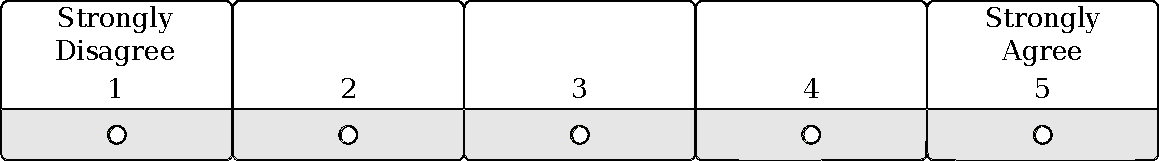
\includegraphics[width=0.65\textwidth]{sus_responses_example.pdf}
\caption{The \ac{sus} response format~\citep{vt100}.}
\label{fig:sus_responses_example}
\end{figure}


\begin{table}
 \caption{Example of a completed \ac{sus} questionnaire. Total score = 22;
 \ac{sus} Score = 22 * 22.5 = 55}
 \label{tbl:sus_results}
 \footnotesize
 \centering
\begin{tabular}{l c c c c c c}
  & \multicolumn{5}{c}{}\\
  & \begin{rotate}{60}\textbf{Strongly disagree}\end{rotate} & & & & 
\begin{rotate}{60}\textbf{Strongly agree}\end{rotate} \\
  \footnotesize
  1. I think that I would like to use this system frequently. 	& {\huge 
\Square} & {\huge \Square} & {\huge \Square} & {\huge \Square} & {\huge 
\CheckedBox}\\
  2. I found the system unnecessarily complex.& {\huge \Square} & {\huge 
\Square} & {\huge \Square} & {\huge \CheckedBox} & {\huge \Square}\\
  3. I thought the system was easy to use.& {\huge \Square} & {\huge 
\CheckedBox} & {\huge \Square} & {\huge \Square} & {\huge \Square}\\
  4. I think that I would need the support of a technical & {\huge \CheckedBox} 
& {\huge \Square} & {\huge \Square} & {\huge \Square} & {\huge \Square}\\
  person to be able to use this system. \\
  5. I found the various functions in this system were well & {\huge \Square} & 
{\huge \CheckedBox} & {\huge \Square} & {\huge \Square} & {\huge \Square}\\
  integrated. \\
  6. I thought there was too much inconsistency in this system.& {\huge \Square} 
& {\huge \Square} & {\huge \CheckedBox} & {\huge \Square} & {\huge \Square}\\
  7. I would imagine that most people would learn to use & {\huge \Square} & 
{\huge \CheckedBox} & {\huge \Square} & {\huge \Square} & {\huge \Square}\\
  this system very quickly. \\
  8. I found the system very cumbersome to use.& {\huge \Square} & {\huge 
\Square} & {\huge \Square} & {\huge \CheckedBox} & {\huge \Square}\\
  9. I felt very confident using the system.& {\huge \Square} & {\huge \Square} 
& {\huge \Square} & {\huge \Square} & {\huge \CheckedBox}\\
  10. I needed to learn a lot of things before I & {\huge \Square} & {\huge 
\Square} & {\huge \CheckedBox} & {\huge \Square} & {\huge \Square}\\
  could get going with this system. \\
\end{tabular}
\end{table}

Although there are other interesting questionnaires (i.e., \ac{sumi}~\citep{sumi},
\ac{mumms}~\citep{mumms}, \ac{quis}~\citep{quis}, and so on), the \ac{sus} 
questionnaire has become an industry standard with references in over 600 
publications~\citep{measuringusability}.

For this evaluation, and along with the \ac{sus} questionnaire, several extra 
questions have been added. The purpose of these questions is to segment the 
whole users set into different subsets of users under similar conditions. Thus, 
three extra classifications have been performed following the following 
criteria:

\begin{itemize}
  \item By age. The users of AdaptUI might encounter different difficulties when
  dealing with the adaptation platform. For example, users older than 65 may not
  be used to use smart devices or touching screens. As is shown through the 
  following charts, age and technology experience are related. To be aware of
  this issue an age based classification has been performed. The subgroups for
  this age classification are:
  \begin{itemize}
    \item Users aged under 20 years old ($x < 20$)\footnote{The $x$ represents
    the age of the user. In this case the $x$ is also shown in the following 
charts
    during this section in the Legend.}.
    \item Users aged between 20 and 35 years old ($20 \leq x < 35$).
    \item Users aged between 35 and 50 years old ($35 \leq x < 50$).
    \item Users aged between 50 and 65 years old ($50 \leq x < 65$).
    \item Users aged over 65 years old ($x > 65$).
  \end{itemize}

  \item By experience with technology. As it might happen with age, the 
  technology experience of the users might result into different usability 
  experiences when using AdaptUI. Touching screens, smart devices, or even 
  technical computer related instructions may be complex depending on the user 
  experience. Hence, a simple classification considering this problem is made 
  with the following criteria:
  
  \begin{itemize}
    \item Low, which indicates a user who is not very familiar with technology.
    This kind of users require non technical further explanations of the AdaptUI
    features, purpose and characteristics. Besides, several \ac{sus} questions might
    trouble these users. Thus, it is desirable to accompany them through the
    \ac{sus} process.
  
    \item Medium, which means that the user usually interacts with technology
    and understands the most common interaction processes and technical 
    vocabulary. Nevertheless, too technical instructions and features might 
    confuse them.
    
    \item High, which characterize those users who have high level technical
    knowledge due to their jobs, hobbies, age, and so forth. These users do not require
    extra explanations or guidelines.
  \end{itemize}
  
  \item By disability. Users are asked if they sense that they might suffer from
  visual or hearing disabilities. Problems when dealing with devices under 
  certain context conditions are included. On the contrary, no specific visual 
  or hearing disability is concreted. The idea is to capture the feeling of 
  the users when manipulating devices under certain conditions (due context 
  or due their own capabilities).
\end{itemize}

Hence, before beginning with the \ac{sus} questionnaire, the following 4 questions
are presented, allowing users to select the corresponding responses through
several combo boxes:

\begin{enumerate}[label=\alph*)]
  \item Please select your age within the following ranges.
  \item Which would you say your experience with technology level is?
  \item Do you feel that, sometimes, you cannot use your mobile device as you
  would like due to a temporary or enduring visual problem? This problem might
  be caused by physiological or context conditions.
  \item Do you feel that, sometimes, you cannot use your mobile device as you
  would like due to a temporary or enduring hearing problem? This problem might
  be caused by physiological or context conditions.
\end{enumerate}

Besides, after these and the \ac{sus} questions two extra questions are presented
regarding developers feedback. The responses are requested through several
check boxes:

\begin{enumerate}[label=\alph*)]
  \item I am a software developer and I usually work with user interfaces.
  \item Considering that I am a developer, I would find the AdaptUI \ac{api} very
  helpful to ease the adaptation of user interfaces.
\end{enumerate}


\subsection{Discussion}
\label{sec:user_evaluation_discussion}

After using AdaptUI and checking its adaptation capabilities, users have been 
asked to complete the \ac{sus} questionnaire with several extra questions. This 
test has been completed by a total of 30 users. Classified into different groups
regarding their age, technology experience and temporary or enduring disabilities 
the obtained results are explained in the following lines illustrated with several 
figures and charts.

First, without considering any of the cited classification criteria, the 
usability results regarding the AdaptUI adaptation system is illustrated through
Figure~\ref{fig:sus_responses}. This figure shows that the 69.56\% of the users
punctuated AdaptUI with over 70 within the \ac{sus} scale. On the contrary, 
approximately the 30\% of the users find its usability under 70 points.

\begin{figure}
\centering
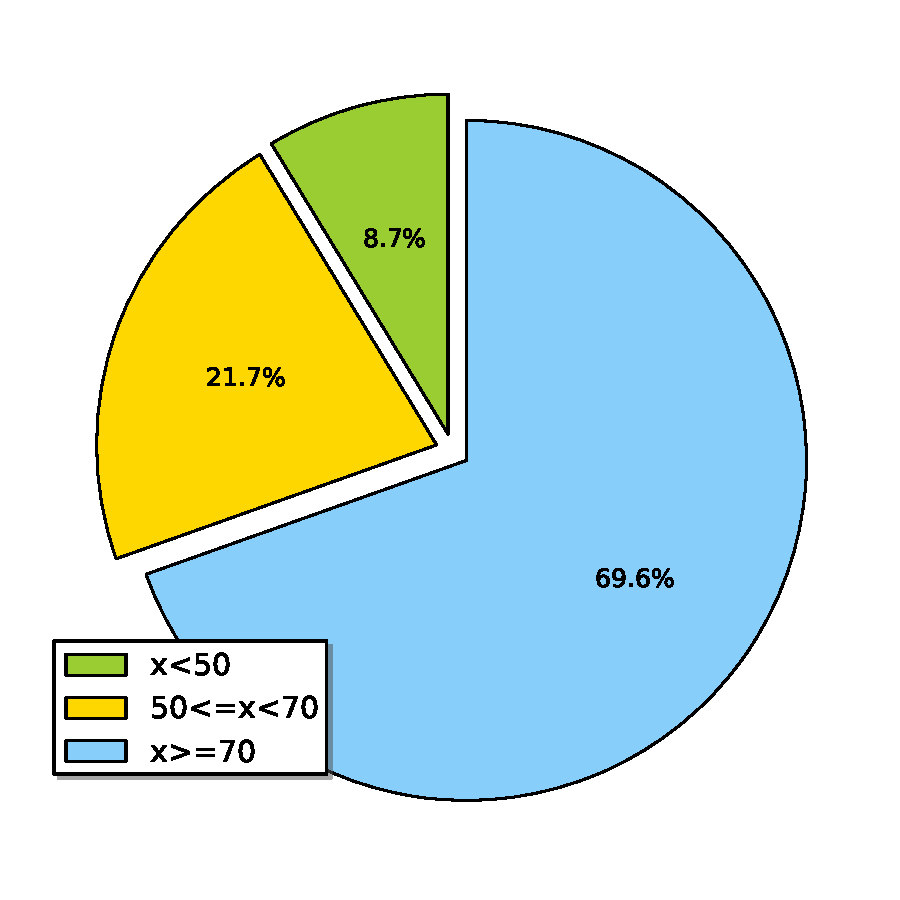
\includegraphics[width=0.65\textwidth]{sus_responses.pdf}
\caption{The \ac{sus} responses.}
\label{fig:sus_responses}
\end{figure}

Next, the cited criteria regarding age, technology experience and possible
disabilities result in the following bar charts. The Figure~\ref{fig:sus_age}
illustrates the differences regarding the \ac{sus} results taking into account the
users ages. In this chart is clearly shown how users between 20 and 35 years old
are the ones who mostly support the AdaptUI usability results. The 43.47\% of
these users consider that the usability of AdaptUI is over 70 in the \ac{sus} scale.

\begin{figure}
\centering
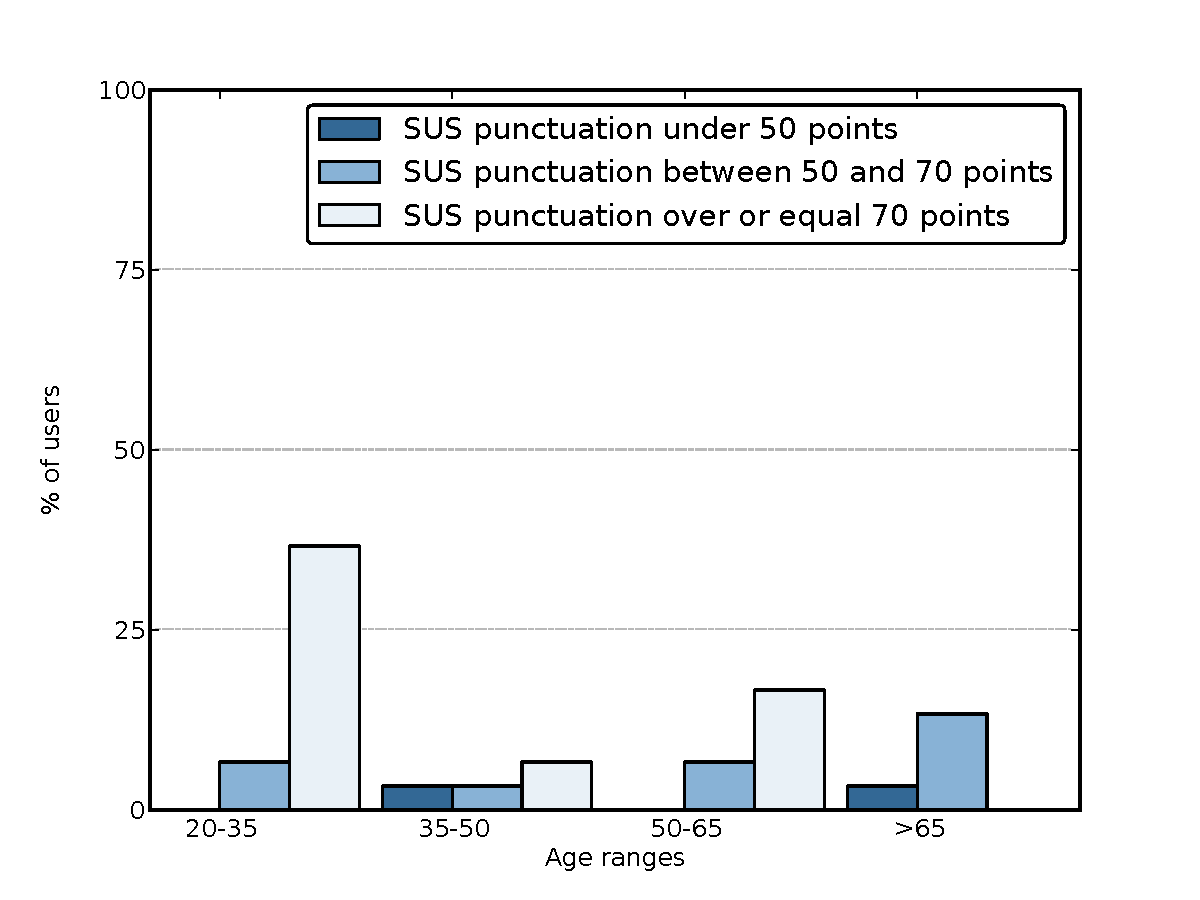
\includegraphics[width=0.65\textwidth]{sus_ages.pdf}
\caption{The \ac{sus} responses taking into account the age range of the users.}
\label{fig:sus_age}
\end{figure}

Along with the age, usually the experience with technology is directly related.
To have this into account, Figure~\ref{fig:sus_experience} illustrates the
resulting differences encountered after analysing the responses given to the \ac{sus}
questionnaire. As is shown, users with \textit{high} technology experience 
result into bigger usability results, reaching a final result of 43.47\% of 
users punctuating AdaptUI over 70 points in the \ac{sus} scale. On the opposite side 
there are those users who lack technology experience. The 8.69\% of these 
users gave less than 50 points. 

\begin{figure}
\centering
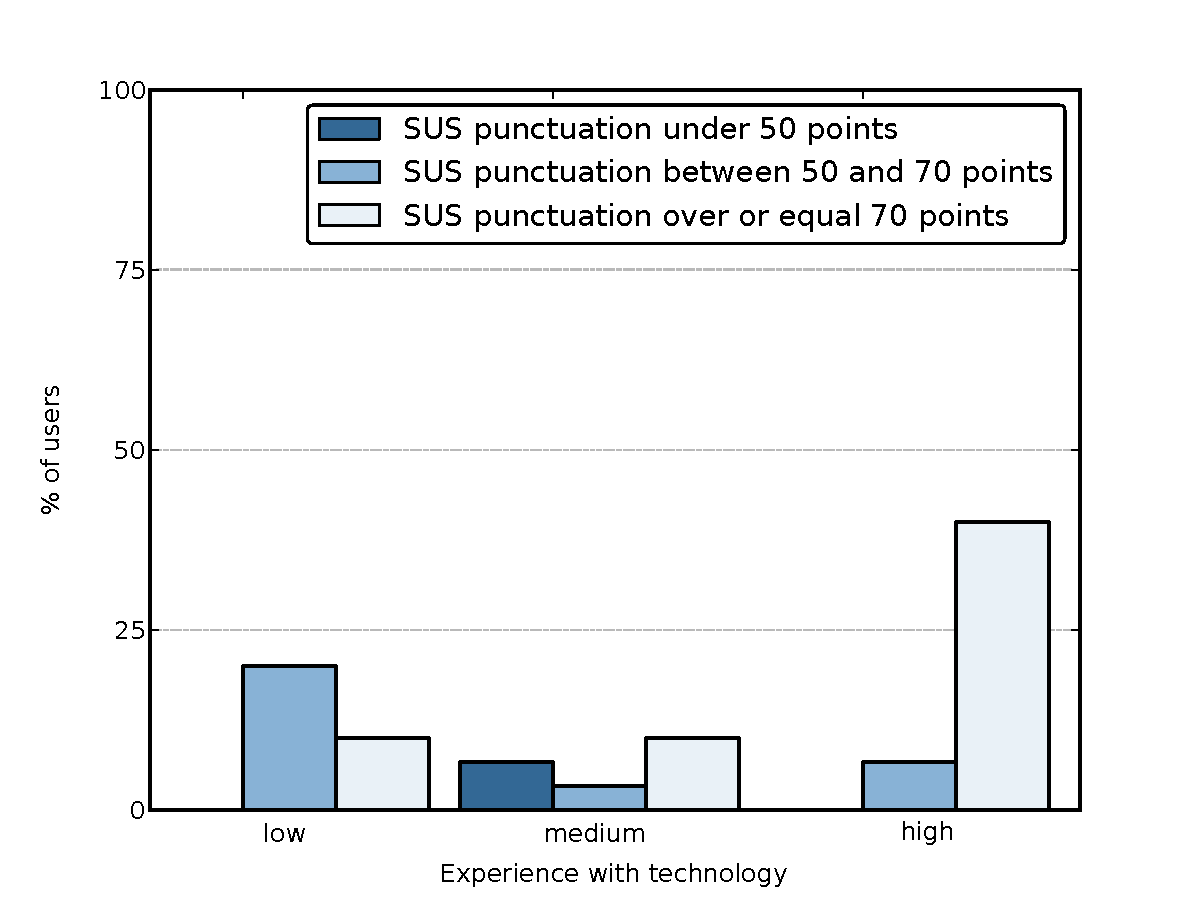
\includegraphics[width=0.65\textwidth]{sus_experience.pdf}
\caption{The \ac{sus} responses taking into account the experience with technology
of the users.}
\label{fig:sus_experience}
\end{figure}

Besides, users are asked about possible disabilities. These disabilities do not
have to be physiological. They are related with the feeling of disability that
users might sense, caused by the context under certain conditions or caused by
other factors. Every user is asked about any possible disability when dealing
with interaction with their devices. As AdaptUI does not consider physiological
capabilities, the users are not asked about this kind of issues directly. The
obtained results show how the 100\% of the asked users with visual or hearing
disabilities find AdaptUI totally usable, punctuating it in the \ac{sus} scale over
70.

\begin{figure}
\centering
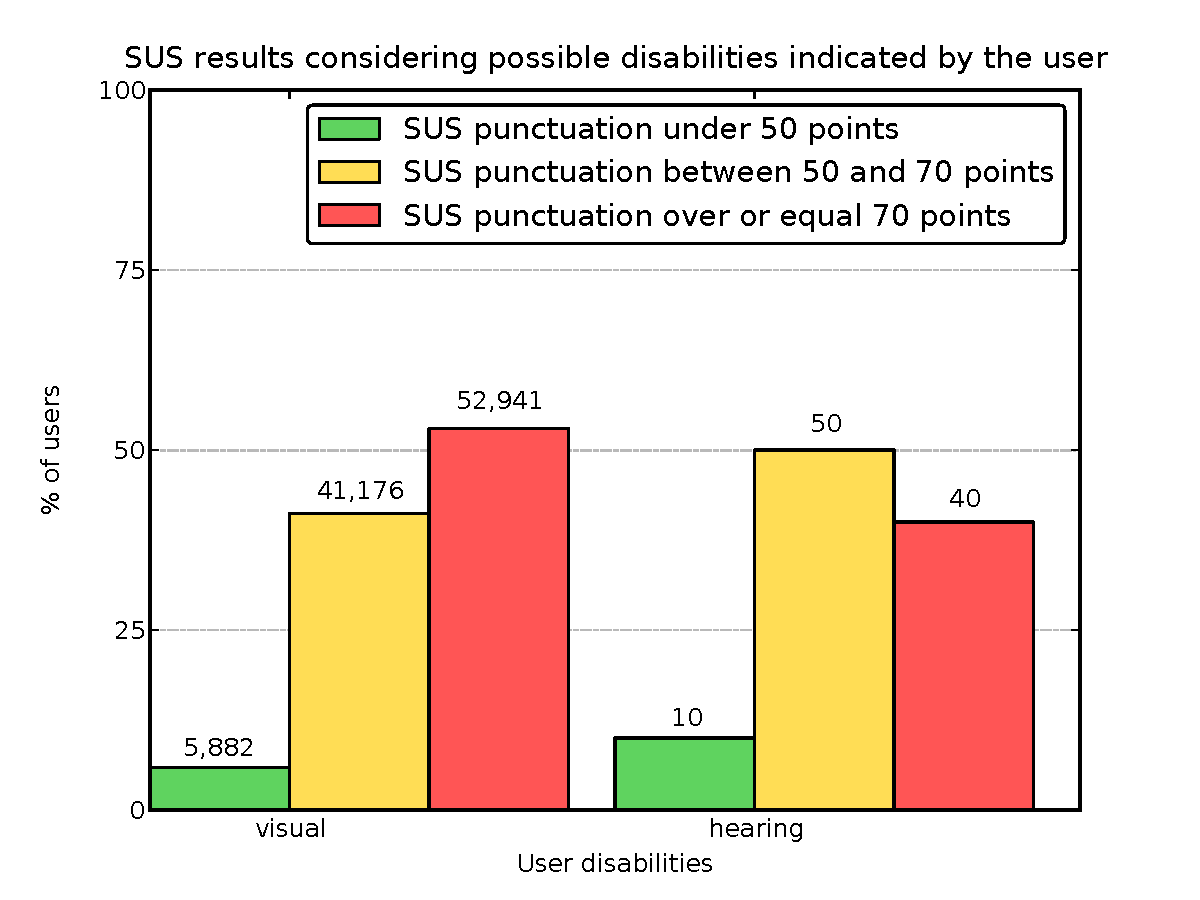
\includegraphics[width=0.65\textwidth]{sus_disability.pdf}
\caption{The \ac{sus} responses taking into account the visual and hearing 
disabilities
indicated by the users.}
\label{fig:sus_disability}
\end{figure}

Finally, we have distinguished between potential users and those who have
development knowledge. In the first versions of the questionnaire this was not
taken into account. However, several evaluations revealed that many users with 
developer profiles stated that they might not find AdaptUI useful as users. On
the contrary, they were willing to use it as developers due to the user 
interface adaptation capabilities of the platform. The 100\% of the users that 
consider themselves developers stated that they would like to use the platform. 
However, Figure~\ref{fig:sus_developers} shown how only the 66.67\% of these 
punctuate AdaptUI with a value of over 70 in the \ac{sus} scale. On the other side, 
the 22.22\% of the developers stated a value between 50 and 70.

\begin{figure}
\centering
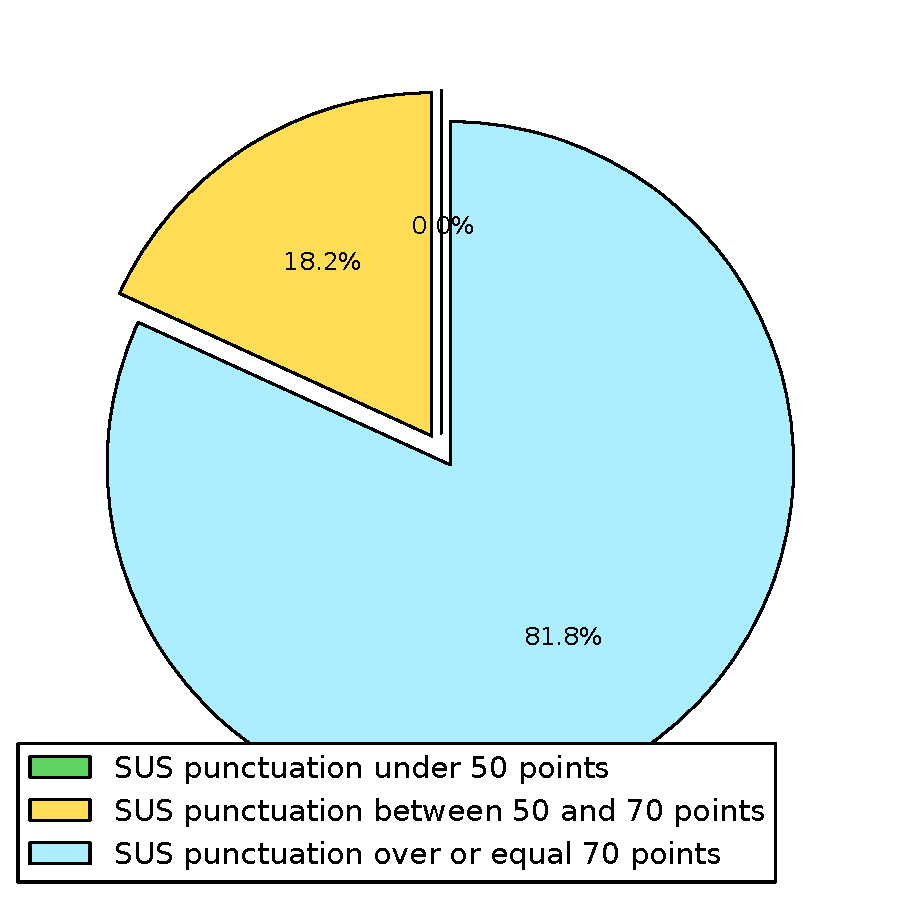
\includegraphics[width=0.65\textwidth]{sus_developers.pdf}
\caption{The \ac{sus} responses taking into account if users are developers.}
\label{fig:sus_developers}
\end{figure}

\subsection{Conclusions}
\label{sec:user_evaluation_conclusions}

Reviewing the results obtained during the user evaluation, several conclusions 
are extracted. In the following lines we summarize these conclusions taking into 
account the segmentation of users by age, experience with technology, possible 
or temporary disabilities, and developer users:

\begin{itemize}
  \item Users ageing is fundamental when dealing with AdaptUI for the first 
  time. While users under 35 years old seem very intuitive and understand most
  of the features and terminology easily, older users usually need more 
  high-level explanations. More precisely, the 43.47 of the users ageing between
  20 and 35 support AdaptUI with more than 70 points in the \ac{sus} scale. On the 
  contrary there are the users ageing over 65 years old. In this case, no one
  gave more than 70 points in the \ac{sus} scale. This is mostly because they 
  encountered several difficulties to understand not only the purpose of the
  system but also the features it provides, and the used and required 
  terminology. This is perceptible through Figure~\ref{fig:sus_age}.
  
  \item The experience with technology, highly associated with ageing, also 
  indicates more or less skill when using the AdaptUI system. Experienced users
  not only understand the features provided by AdaptUI, but they also predict
  the results of the experiments or even contribute with possible features to 
  cover they daily experiences with user interfaces. As is illustrated through
  Figure~\ref{fig:sus_experience}, the 43\% of the users with \textit{high} 
  experience with technology gave to AdaptUI more than 70 points in the 
  usability scale. Contrarily, the 8\% of the \textit{low} experienced users 
  the same punctuation.
  
  \item Regarding the possible disabilities we might suffer from when 
  manipulating our devices in different contexts, users are very comfortable 
  with the purpose of AdaptUI. Nevertheless, in this point we encountered 
  several differences. For example, a significant percentage of users that are
  also developers find the AdaptUI \ac{api} more interesting than the scenarios. 
  In other words, they prefer using AdaptUI as a framework for their applications
  than using it for their daily lives as mobile devices users. Focusing on the
  results, Figure~\ref{fig:sus_disability} shows similar outcomes considering
  both visual and hearing disabilities. In the first case the 63.63\% of the 
  users gave more than 70 points, while in the second case the percentage is 
  57.14\%.
  
  \item Finally, regarding the results obtained from users who are also 
  developers, we find that the 72.72\% of these users find AdaptUI usable, 
  giving 70 or more points in the \ac{sus} scale. The rest of developer users 
  stated that they find AdaptUI a necessary platform for the inclusive design of 
  the user interface of their applications, expressing that, as users (not 
  developers), they might not use AdaptUI. These outcomes are illustrated
  through Figure~\ref{fig:sus_developers}.
\end{itemize}

In general terms the acceptance of AdaptUI regarding usability and developer
needs is promising. As Figure~\ref{fig:sus_responses} shows, the 69.56\% of all 
the users find AdaptUI usable over 70 usability points. On the contrary only
the 8.69~\% gave less than 50 points. Nevertheless, and as is detailed in 
Section~\ref{sec:future_work}, more efforts are planned to try to get better
results for both users and developers.